% Informe final (versión en español): demosaicking multiespectral agnóstico
% al patrón. Traducción de report.tex.
% Basado en la plantilla ICIP 2026; se usa con:
%          spconf.sty  - estilo LaTeX de ICASSP/ICIP, y
%          IEEEbib.bst - estilo bibliográfico IEEE.
% Todas las cifras vienen de ../results/ (summary.csv, per_scene.csv,
% hypotheses.json), de ../results_arad/ (protocolo entre conjuntos de datos,
% Sección 5.4) o de las pruebas cortas de scripts/pilot.py (ablación). Las figuras vienen de
% ../results/figs_es/ (python -m msdemosaic.figures --data-mode cave-split --lang es).
% Compilar desde esta carpeta:  tectonic informe.tex
% --------------------------------------------------------------------------
\documentclass{article}
\usepackage[hyphens]{url}
\usepackage{spconf,amsmath,amssymb,graphicx,tikz,array,multirow}
\usepackage[spanish,es-noshorthands,es-tabla,es-nodecimaldot,es-nolists]{babel}
% spconf pide Times (ptm), que no existe con XeTeX/tectonic: sin esto la
% negrita y la cursiva no se ven. TeX Gyre Termes es un clon de Times.
\usepackage{fontspec}
\setmainfont{texgyretermes}[Extension=.otf, UprightFont=*-regular,
  BoldFont=*-bold, ItalicFont=*-italic, BoldItalicFont=*-bolditalic]
\setmonofont{lmmono10-regular.otf}
\newcolumntype{L}[1]{>{\raggedright\arraybackslash}p{#1}}
\newcolumntype{C}[1]{>{\centering\arraybackslash}p{#1}}
\usetikzlibrary{arrows.meta,positioning,fit}
\graphicspath{{../results/figs_es/}}

% Encabezados de spconf en español (la plantilla los tiene fijos en inglés).
\makeatletter
\def\abstract{\begin{center}
{\bf RESUMEN\vspace{-.5em}\vspace{0pt}}
\end{center}}
\def\keywords{\vspace{.5em}
{\bfseries\textit{Palabras clave}---\,\relax%
}}
\def\thebibliography#1{\section{Referencias}\list
 {[\arabic{enumi}]}{\settowidth\labelwidth{[#1]}\leftmargin\labelwidth
 \advance\leftmargin\labelsep
 \usecounter{enumi}}
 \def\newblock{\hskip .11em plus .33em minus .07em}
 \sloppy\clubpenalty4000\widowpenalty4000
 \sfcode`\.=1000\relax}
\def\fnum@table{{\bf Tabla \thetable}}
\makeatother

% Notación.
% ---------
\def\X{{\mathbf X}}
\def\Y{{\mathbf Y}}
\def\C{{\mathbf C}}
\def\M{{\mathbf M}}
\def\N{{\mathbf N}}
\def\x{{\mathbf x}}
\newcommand{\wb}{\mathrm{WB}}
\newcommand{\seen}[1]{\underline{#1}}

% Paleta espectral para dibujar los patrones MSFA (banda 1 = violeta, 16 = rojo).
\definecolor{b1}{HTML}{5B3FD0}\definecolor{b2}{HTML}{4F4FD8}
\definecolor{b3}{HTML}{3F62DC}\definecolor{b4}{HTML}{2A75DB}
\definecolor{b5}{HTML}{1E88D0}\definecolor{b6}{HTML}{1A99B8}
\definecolor{b7}{HTML}{1BA49B}\definecolor{b8}{HTML}{2DAE7A}
\definecolor{b9}{HTML}{5BB55A}\definecolor{b10}{HTML}{8FBC40}
\definecolor{b11}{HTML}{C2C036}\definecolor{b12}{HTML}{E3B935}
\definecolor{b13}{HTML}{E8A030}\definecolor{b14}{HTML}{E8822C}
\definecolor{b15}{HTML}{DD5E31}\definecolor{b16}{HTML}{C93A3A}

% \msfa{expr}: dibuja un recorte de 16x16 de un MSFA; expr da la banda (1..16)
% del píxel en la fila \i y la columna \j (ambas desde 0).
\newcommand{\msfa}[1]{%
  \begin{tikzpicture}[x=0.118cm,y=0.118cm]
    \foreach \i in {0,...,15}{
      \foreach \j in {0,...,15}{
        \pgfmathtruncatemacro{\b}{#1}
        \edef\c{b\b}
        \fill[fill=\c] (\j,-\i) rectangle ++(1,-1);
      }
    }
    \draw[black!60, line width=0.3pt] (0,0) rectangle (16,-16);
  \end{tikzpicture}}

% Título.
% -------
\title{UNA RED PARA CUALQUIER ARREGLO DE FILTROS:\\
  DEMOSAICKING MULTIESPECTRAL AGNÓSTICO AL PATRÓN}
%
\name{Benjamín Cisternas, Gonzalo Michea}
\address{Fotografía Computacional 2026-2\\
  Departamento de Informática, Universidad Técnica Federico Santa María\\
  Valparaíso, Chile}
%
\begin{document}
%
\maketitle
%
\begin{abstract}
Las cámaras multiespectrales instantáneas usan un arreglo de filtros
multiespectral (MSFA), por lo que cada píxel mide una de 16 bandas y hay que
estimar cerca del 94\% del cubo de datos. Las redes de demosaicking
aprendidas dan los mejores resultados, pero deben reentrenarse para cada
MSFA. Condicionamos una U-Net pequeña al patrón entregándole una estimación
bilineal, las mediciones dispersas y la máscara, la entrenamos con patrones
aleatorios balanceados y la probamos con cuatro MSFA que nunca vio (IMEC,
empaquetamiento óptimo de esferas, BTES y un kernel aleatorio). En escenas
reservadas de CAVE, las redes entrenadas para un patrón pierden entre 7.4 y
15.5\,dB en los demás patrones y quedan bajo la interpolación bilineal. La
red agnóstica queda entre 1.2 y 1.4\,dB bajo cada red especializada en el
patrón de esa red, y entre 6.3 y 9.9\,dB sobre ellas en patrones no vistos.
Entrenar con ARAD-1K y probar en las 32 escenas de CAVE lleva a las mismas
conclusiones, aunque todos los métodos aprendidos pierden precisión al
cambiar de conjunto de datos.
\end{abstract}
%
\begin{keywords}
Imágenes multiespectrales, arreglo de filtros multiespectral, demosaicking,
aprendizaje profundo, generalización
\end{keywords}
%
% ==========================================================================
\section{Introducción}
\label{sec:intro}
% ==========================================================================

Una cámara a color registra tres valores por píxel, pero el espectro de
reflectancia de la mayoría de los materiales contiene mucha más información
que tres números. Las imágenes multiespectrales (MSI) muestrean el espectro
en varias bandas angostas, típicamente entre 8 y 32 en el rango visible e
infrarrojo cercano. El resultado es un \emph{cubo de datos} con dos
dimensiones espaciales y una espectral. El espectro de cada píxel ayuda a
distinguir materiales que en RGB se ven iguales, por lo que las MSI se usan
en percepción remota~\cite{diaz2023}, imágenes médicas~\cite{lu2014},
agricultura, inspección de alimentos y patrimonio cultural.

Lo difícil de las MSI es la adquisición, porque un sensor 2D no puede
registrar un cubo 3D en una sola exposición sin ceder en algo. Las cámaras
de barrido registran el cubo una línea o una banda a la vez, lo que es lento
y falla con escenas en movimiento. Las cámaras instantáneas basadas en un
\emph{arreglo de filtros multiespectral} (MSFA, por su sigla en inglés)
sacrifican muestreo espacial a cambio de velocidad: un mosaico de filtros de
banda angosta cubre el sensor y cada píxel mide una sola
banda~\cite{lapray2014,geelen2014}. Luego, un algoritmo de
\emph{demosaicking} debe estimar los valores que faltan. Con $L=16$ bandas,
cada banda se mide en solo $1/16$ de los píxeles, así que se desconoce cerca
del 94\% del cubo, mucho más que en el demosaicking RGB, donde el verde se
mide en la mitad de los píxeles. Por eso la calidad de imagen de una cámara
MSFA depende tanto del algoritmo de demosaicking como del sensor.

Dos líneas de investigación han mejorado las cámaras MSFA. La primera
diseña mejores patrones: Diaz et al.~\cite{diaz2023} ubicaron hace poco los
filtros mediante \emph{empaquetamiento óptimo de esferas} (OSP) en el
dominio espacio-espectral y reportaron hasta 2\,dB de mejora respecto de
siete MSFA existentes. La segunda aprende la reconstrucción con redes
neuronales convolucionales, que superan con claridad a la interpolación
clásica~\cite{feng2021,diaz2023}. Las dos líneas no se combinan con
facilidad. Una red que recibe solo el mosaico aprende el patrón de forma
implícita y queda atada al MSFA de entrenamiento. En~\cite{diaz2023} la red
se reentrenó para cada patrón, cerca de un día y medio en dos GPU cada vez,
y los autores reconocen que ``una limitación importante del método propuesto
es la necesidad de reentrenar para MSFA específicos'' (traducción nuestra).
Comparar $n$ patrones candidatos exige entonces $n$ redes entrenadas, y una
cámara con un patrón nuevo o levemente distinto necesita un modelo nuevo.

\textbf{Pregunta de investigación.} \emph{¿Puede una sola red de
demosaicking reconstruir imágenes multiespectrales con cualquier MSFA,
incluso con patrones que no vio durante el entrenamiento, con una calidad
cercana a la de una red entrenada para cada patrón?} Ponemos a prueba tres
hipótesis:
\begin{itemize}
  \item[\textbf{H1}] Una red entrenada para un patrón se degrada
        fuertemente en patrones no vistos.
  \item[\textbf{H2}] Una red agnóstica al patrón queda a menos de 2\,dB de
        cada red específica en el patrón propio de esa red. Nuestra
        propuesta escrita usaba un umbral más estricto de 1\,dB; reportamos
        ambos.
  \item[\textbf{H3}] En patrones no vistos, la red agnóstica supera tanto a
        las redes específicas como a la interpolación bilineal.
\end{itemize}

\textbf{Contribuciones.} (i) Un flujo abierto en Python para simular y
evaluar demosaicking MSFA, verificado con el código público
de~\cite{diaz2023}: nuestros patrones coinciden píxel a píxel con los suyos
y nuestra interpolación bilineal ponderada reproduce su PSNR con 0.13\,dB de
diferencia. (ii) Una medición sistemática de cuánto depende el demosaicking
aprendido del patrón de entrenamiento. (iii) Una red agnóstica al patrón
para MSFA de 16 bandas: una U-Net condicionada al patrón a través de su
entrada y entrenada con patrones aleatorios balanceados. Esto extiende el
entrenamiento con patrones aleatorios, ya mostrado para arreglos de filtros
RGB~\cite{bourrier2022}, a un caso con 94\% de valores faltantes en vez de
dos tercios. (iv) Una ablación de la entrada de la red. La mayor parte de la
ganancia viene de entregarle una interpolación que conoce el patrón; sin
ella, la red agnóstica queda bajo la interpolación bilineal con el mismo
presupuesto de entrenamiento. (v) Un experimento entre conjuntos de datos
(entrenar con ARAD-1K y probar en las 32 escenas de CAVE) que repite la
comparación con cuatro veces más escenas de prueba.

% ==========================================================================
\section{Antecedentes y trabajo relacionado}
\label{sec:background}
% ==========================================================================

\subsection{Formación de la imagen}

Denotamos el cubo por $\X\in\mathbb{R}^{H\times W\times L}$. Su banda $k$,
$\X_k\in\mathbb{R}^{H\times W}$, es la escena vista a través de un filtro
angosto centrado en la longitud de onda $\lambda_k$, y
$\x(m,n)\in\mathbb{R}^L$ es el espectro en el píxel $(m,n)$. Un MSFA asigna
una banda a cada píxel. Sea $\C_k\in\{0,1\}^{H\times W}$ la máscara binaria
de la banda $k$, con $\sum_k\C_k=\mathbf{1}$. Con filtros ideales de banda
angosta, el sensor registra el mosaico~\cite{diaz2023}
\begin{equation}
  \Y = \sum_{k=1}^{L} \X_k \odot \C_k + \N,
  \label{eq:model}
\end{equation}
donde $\odot$ es el producto elemento a elemento y $\N$ es el ruido del
sensor. La máscara \emph{one-hot}
$\M=[\C_1,\dots,\C_L]\in\{0,1\}^{H\times W\times L}$ describe por completo
el patrón, y $\Y\odot\M$ (con $\Y$ replicado en las bandas) es el
\emph{cubo disperso}, que pone cada medición en su propia banda. El
demosaicking estima $\X$ a partir de $\Y$. La Ec.~\eqref{eq:model} da $HW$
ecuaciones para $HWL$ incógnitas, así que el problema está muy mal planteado
y todo método necesita un modelo previo de las imágenes naturales. Los más
usados son la correlación espacial (los píxeles vecinos se parecen) y la
espectral (las bandas de longitudes de onda cercanas se parecen). Cuando ese
modelo falla, los artefactos típicos son patrones \emph{zipper} que siguen
el período del kernel de filtros, \emph{colores falsos} (espectros que no
existen en la escena) y desenfoque~\cite{diaz2023}.

\subsection{Diseño de MSFA}

Igual que el arreglo de Bayer~\cite{bayer1976}, la mayoría de los MSFA
repite un kernel pequeño. Por ejemplo, los sensores comerciales de IMEC
teselan un kernel de $4\times4$ con 16 bandas~\cite{geelen2014}. Otros
diseños son los kernels aleatorios (RND) y secuenciales, el patrón de
Brauers y Aach~\cite{brauers2006} y el patrón BTES (\emph{binary-tree-based
edge-sensing})~\cite{miao2006}. Hirakawa y Wolfe~\cite{hirakawa2008} dieron
uno de los primeros criterios formales, en el dominio de Fourier, para
arreglos de filtros de color. Diaz et al.~\cite{diaz2023} representan cada
píxel muestreado como un punto (fila, columna, banda) en un cubo de
$L\times L\times L$ y buscan puntos lo más separados posible, lo que es un
problema de empaquetamiento de esferas. En la grilla del sensor restringen
la búsqueda a retículas
\begin{equation}
  B(i,j) = \big((a\,i + b\,j)\bmod L\big) + 1,
  \label{eq:osp}
\end{equation}
donde $i,j$ son los índices de fila y columna contados desde 1. El mejor par
para $L=16$ es $a=7$, $b=4$. Este patrón OSP tiene un diámetro de esfera de
2.45 y una densidad de empaquetamiento de 0.40, contra 1.41 y 0.08 de IMEC
y 1.73 y 0.14 de BTES~\cite{diaz2023}. OSP se repite cada 16 filas y cada 4
columnas, así que, a diferencia de IMEC y BTES, no es un kernel de
$4\times4$ teselado. La Fig.~\ref{fig:patterns} muestra los cuatro patrones
usados en este trabajo.

\begin{figure}[t]
\centering
\begin{minipage}[b]{0.24\linewidth}
  \centering
  \msfa{{7,8,6,5,15,16,14,13,11,12,10,9,3,4,2,1}[4*mod(\i,4)+mod(\j,4)]}
  \centerline{\small (a) IMEC}
\end{minipage}\hfill
\begin{minipage}[b]{0.24\linewidth}
  \centering
  \msfa{mod(7*(\i+1)+4*(\j+1),16)+1}
  \centerline{\small (b) OSP}
\end{minipage}\hfill
\begin{minipage}[b]{0.24\linewidth}
  \centering
  \msfa{{1,13,4,15,9,5,11,7,3,16,2,14,12,8,10,6}[4*mod(\i,4)+mod(\j,4)]}
  \centerline{\small (c) BTES}
\end{minipage}\hfill
\begin{minipage}[b]{0.24\linewidth}
  \centering
  \msfa{{11,3,14,6,1,9,16,4,13,7,2,12,5,15,8,10}[4*mod(\i,4)+mod(\j,4)]}
  \centerline{\small (d) Aleatorio}
\end{minipage}
\caption{Recortes de $16\times16$ de los cuatro MSFA de prueba con $L=16$
(color = banda, de violeta en 400\,nm a rojo en 700\,nm). (a) Kernel IMEC de
$4\times4$~\cite{geelen2014}; (b) retícula de empaquetamiento de esferas de
la Ec.~\eqref{eq:osp} con $a=7$, $b=4$~\cite{diaz2023};
(c) BTES~\cite{miao2006}; (d) un kernel aleatorio fijo de $4\times4$.
(a)--(c) coinciden píxel a píxel con el código público de~\cite{diaz2023}.}
\label{fig:patterns}
\end{figure}

\subsection{Demosaicking clásico}

La interpolación \textbf{bilineal ponderada (WB)}~\cite{brauers2006}
interpola cada banda dispersa $\Y\odot\C_k$ por separado con un kernel
pasabajos normalizado. Es rápida e independiente del patrón, pero ignora la
correlación espectral y desenfoca los bordes. Los métodos de
\textbf{diferencia espectral} interpolan la diferencia entre dos bandas, que
es más suave, en lugar de las bandas mismas~\cite{brauers2006,mizutani2014}.
Los métodos \textbf{guiados por intensidad} estiman primero una imagen que
combina todas las bandas, como la imagen pseudo-pancromática de
PPID~\cite{mihoubi2017}, e interpolan cada banda respecto de ella. El
demosaicking también se puede plantear como un problema inverso
regularizado, por ejemplo con modelos de bajo rango y de
grafos~\cite{tsagkatakis2019}.

\subsection{Demosaicking aprendido}

Una red $f_\theta$ se entrena con pares $(\Y,\X)$ simulados con la
Ec.~\eqref{eq:model} a partir de cubos capturados con cámaras de barrido.
Algunos ejemplos son la red de convolución y atención para mosaicos
(MCAN)~\cite{feng2021} y TRevSCI~\cite{diaz2023}, una adaptación de una red
reversible para imágenes compresivas instantáneas~\cite{cheng2021}. En RGB,
Gharbi et al.~\cite{gharbi2016} mostraron que hacer demosaicking y quitar el
ruido con una sola red funciona mejor que resolver ambos pasos por separado.
El desafío NTIRE 2022 de demosaicking espectral~\cite{arad2022demosaic}
comparó métodos aprendidos en imágenes MSFA de 16 canales.
En~\cite{diaz2023}, TRevSCI mejora a WB en 5 a 8\,dB, pero recibe solo $\Y$
y se reentrenó para cada uno de los ocho MSFA estudiados.

\subsection{Demosaicking independiente del patrón}

Para arreglos de filtros de color (CFA) RGB hay varios métodos que funcionan
con cualquier patrón. Zhang et al.~\cite{zhang2016} propusieron un método
clásico de demosaicking universal para CFA periódicos y aperiódicos, y
Stojkovi\'c et al.~\cite{stojkovic2019} usaron algoritmos independientes del
CFA para comparar distintas disposiciones. Henz et al.~\cite{henz2018}
aprenden el CFA junto con la red, que luego queda atada al patrón aprendido.
Lo más cercano a nuestro trabajo es Bourrier et al.~\cite{bourrier2022}, que
entrenaron una CNN con imágenes RGB con mosaicos aleatorios y observaron que
funciona igual de bien en mosaicos periódicos y en otros mosaicos
aleatorios. Bai et al.~\cite{bai2024} tratan CFA dispersos arbitrarios con
una red cuya primera operación es una interpolación ponderada de las
muestras. Para MSFA, los métodos genéricos son sobre todo clásicos: WB y
PPID funcionan con cualquier patrón, y Bian et al.~\cite{bian2021}
propusieron un método no local de bajo rango generalizado, y señalan que los
métodos existentes tienen precisión limitada o generalizan mal. Wang y
Davies~\cite{wang2026} describieron hace poco un método multiespectral
autosupervisado que no depende de un patrón específico, pero lo evalúan con
un solo MSFA de $4\times4$.

Tomamos además dos ideas de otros problemas. La \emph{convolución
normalizada}~\cite{knutsson1993} filtra las muestras dispersas y divide por
la máscara filtrada, así que el mismo operador sirve para cualquier
disposición de muestras; WB con un kernel normalizado es un caso particular.
Las \emph{convoluciones parciales}~\cite{liu2018} condicionan una red de
\emph{inpainting} a una máscara de huecos arbitraria, y la red se entrena con
máscaras aleatorias para que generalice a máscaras nuevas. Nosotros
aplicamos patrones aleatorios y una entrada que incluye la máscara a MSFA de
16 bandas. Hasta donde sabemos, nadie había medido de forma sistemática cómo
generaliza el demosaicking MSFA aprendido a patrones no vistos.

% ==========================================================================
\section{Método propuesto}
\label{sec:method}
% ==========================================================================

\subsection{Entrada de la red}

Una red de demosaicking convencional calcula $\hat\X=f_\theta(\Y)$. Como el
patrón no es una entrada, la red solo puede aprenderlo de los datos de
entrenamiento. Nosotros, en cambio, condicionamos la red al patrón a través
de su entrada:
\begin{equation}
  \hat\X = f_\theta\big(\,[\,\wb(\Y,\M),\;\Y\odot\M,\;\M\,]\,\big),
  \label{eq:input}
\end{equation}
donde $[\cdot]$ concatena en el eje de canales, lo que da $3L=48$ canales de
entrada. Cada parte cumple un papel distinto:
\begin{itemize}
  \item $\wb(\Y,\M)$ es una primera estimación del cubo completo que ya
        depende del patrón. La calculamos por convolución
        normalizada~\cite{knutsson1993}: para cada banda $k$,
        \begin{equation}
          \wb_k = \frac{K * (\Y\odot\C_k)}{K * \C_k},
          \label{eq:wb}
        \end{equation}
        donde $K$ es el kernel triangular separable de $7\times7$ construido
        a partir de $(1,2,3,4,3,2,1)$, como en el código WB
        de~\cite{diaz2023}. Los píxeles medidos conservan su valor. La
        Ec.~\eqref{eq:wb} sirve para cualquier patrón, incluso no periódico,
        y normaliza bien en los bordes de la imagen.
  \item $\Y\odot\M$ entrega los valores medidos exactos, cada uno en su
        banda.
  \item $\M$ le indica a la red qué valores se midieron y cuáles se
        interpolaron.
\end{itemize}
Con esta entrada la red no tiene que averiguar desde cero a qué banda
pertenece cada píxel. Recibe una interpolación que ya depende del patrón y
aprende a corregirla con las correlaciones espaciales y espectrales. En
nuestra ablación (Sección~\ref{sec:ablation}) esta fue la decisión que más
pesó: con la entrada de nuestro plan de proyecto, $[\Y,\M]$, la red aprendía
varias veces más lento.

\subsection{Arquitectura y función de pérdida}

$f_\theta$ es una U-Net~\cite{ronneberger2015} pequeña con dos niveles de
submuestreo. Cada nivel tiene dos convoluciones de $3\times3$ con ReLU, con
48, 96 y 192 canales de arriba hacia abajo. Se usa \emph{max pooling} para
submuestrear, convoluciones transpuestas para sobremuestrear y conexiones de
salto entre cada nivel del codificador y el nivel correspondiente del
decodificador. Una convolución final de $1\times1$ entrega directamente las
16 bandas. No hay capas de normalización ni conexión residual. La red tiene
1\,068\,640 parámetros y es totalmente convolucional, así que acepta
imágenes de cualquier tamaño (las entradas se rellenan hasta un múltiplo
de 4). Como en~\cite{diaz2023}, minimizamos la pérdida $\ell_1$,
$\|\hat\X-\X\|_1$.

\subsection{Patrones de entrenamiento}

Lo único que distingue a una red específica de la red agnóstica es el
conjunto de patrones que ve durante el entrenamiento. Una red específica
siempre ve el mismo MSFA. La red agnóstica ve un patrón aleatorio
\emph{balanceado} nuevo en cada lote, en el que cada banda aparece
exactamente una vez en cada bloque alineado de $4\times4$. Se muestrean dos
familias con igual probabilidad:
\begin{itemize}
  \item \emph{Teselada}: una permutación aleatoria de las 16 bandas forma un
        kernel de $4\times4$ que se repite en todo el parche. Se descartan
        los kernels iguales a alguno de los tres kernels teselados de prueba
        (IMEC, BTES y Aleatorio).
  \item \emph{Por bloques}: cada bloque alineado de $4\times4$ recibe su
        propia permutación aleatoria independiente, así que el patrón no
        tiene período.
\end{itemize}
La familia teselada cubre los MSFA basados en kernels. Agregamos la familia
por bloques para los patrones no periódicos, porque OSP no es un kernel de
$4\times4$ teselado. OSP sí tiene una banda por bloque alineado de
$4\times4$, así que en principio la familia por bloques podría generarlo.
Sin embargo, un parche de entrenamiento de $64\times64$ contiene 256
bloques, por lo que la probabilidad de muestrear OSP es $(16!)^{-256}$. En
la práctica, la red agnóstica nunca ve ninguno de los cuatro patrones de
prueba. La Fig.~\ref{fig:method} resume el esquema de entrenamiento.

\begin{figure}[t]
\centering
\begin{tikzpicture}[
    box/.style={draw, rounded corners=2pt, align=center, minimum height=0.85cm,
                font=\footnotesize, inner sep=2.5pt},
    arr/.style={-{Stealth[length=4pt]}, thick}]
  \node[box] (cube) {Cubo\\$\X$};
  \node[box, right=0.38cm of cube] (sim) {Ec.~\eqref{eq:model}};
  \node[box, above=0.3cm of sim] (rand) {Patrón $\M$:\\fijo o aleatorio};
  \node[box, right=0.38cm of sim] (in) {$\wb(\Y,\M)$\\$\Y\odot\M$\\$\M$};
  \node[box, right=0.38cm of in, fill=black!8] (net) {U-Net\\$f_\theta$};
  \node[box, right=0.38cm of net] (out) {$\hat\X$};
  \draw[arr] (cube) -- (sim);
  \draw[arr] (rand) -- (sim);
  \draw[arr] (rand) -| (in);
  \draw[arr] (sim) -- node[above, font=\scriptsize] {$\Y$} (in);
  \draw[arr] (in) -- (net);
  \draw[arr] (net) -- (out);
  \draw[arr, dashed] (out.south) -- ++(0,-0.45) -| node[pos=0.25, below,
       font=\scriptsize] {$\ell_1(\hat\X,\X)$} (cube.south);
\end{tikzpicture}
\caption{Esquema de entrenamiento. En cada lote, el mosaico $\Y$ se simula
con la Ec.~\eqref{eq:model} a partir de un patrón $\M$, que es siempre el
mismo para una red específica y un patrón aleatorio balanceado nuevo para la
red agnóstica. La red recibe la estimación WB, el cubo disperso y la máscara
(Ec.~\eqref{eq:input}).}
\label{fig:method}
\end{figure}

% ==========================================================================
\section{Montaje experimental}
\label{sec:setup}
% ==========================================================================

\textbf{Datos.} CAVE~\cite{yasuma2010} tiene 32 escenas de interior de
$512\times512$ píxeles con 31 bandas de 400 a 700\,nm cada 10\,nm, guardadas
como imágenes de 16 bits que escalamos a $[0,1]$. ARAD-1K~\cite{arad2022}
tiene 950 escenas públicas de entrenamiento de $482\times512$ píxeles con
las mismas 31 bandas, de interior y de exterior, capturadas con otra cámara;
lo obtuvimos de una copia pública~\cite{he2023zenodo}. Como
en~\cite{diaz2023}, conservamos 16 bandas (400, 420, \dots, 700\,nm). Usamos
dos protocolos. En el principal, la \emph{partición de CAVE}, dividimos CAVE
con una permutación aleatoria fija (semilla 0) en 21 escenas de
entrenamiento, 3 de validación y 8 de prueba: \textit{sponges},
\textit{paints}, \textit{fake and real food}, \textit{stuffed toys},
\textit{pompoms}, \textit{beads}, \textit{fake and real tomatoes} y
\textit{watercolors}. En el protocolo \emph{entre conjuntos de datos}
(Sección~\ref{sec:cross}) entrenamos con 220 escenas de ARAD-1K, validamos
con otras 30 y probamos en las 32 escenas de CAVE. Usamos 250 de las 950
escenas para que el conjunto de entrenamiento quepa en la memoria de nuestro
computador portátil. Ninguna escena de prueba se usa para entrenar ni para
elegir modelos.

\textbf{Simulación.} Los mosaicos se simulan con la Ec.~\eqref{eq:model},
filtros ideales y sin ruido ($\N=0$). Todo patrón se ancla en el píxel
superior izquierdo de la imagen o del parche. La Fig.~\ref{fig:patterns}
muestra los cuatro patrones de prueba.

\textbf{Métodos.} Comparamos cinco métodos: (1) \textbf{WB},
Ec.~\eqref{eq:wb}, sin aprendizaje; (2) \textbf{U-Net fija-IMEC} y
(3) \textbf{U-Net fija-OSP}, la red de la Sección~\ref{sec:method} entrenada
solo con IMEC o solo con OSP; (4) \textbf{U-Net agnóstica}, la misma red
entrenada con patrones aleatorios; y (5) \textbf{U-Net sin máscara (IMEC)},
una red convencional que recibe solo $\Y$ (1\,048\,336 parámetros) y se
entrena con IMEC. Los métodos (2) a (4) tienen la misma entrada y
arquitectura, así que cualquier diferencia entre ellos se debe solo a los
patrones de entrenamiento. El método (5) corresponde a la forma habitual de
entrenar redes de demosaicking.

\textbf{Entrenamiento.} Todas las redes se entrenan por 20\,000 iteraciones
con lotes de 32 parches aleatorios de $64\times64$, aumentados con
reflexiones y rotaciones aleatorias de $90^\circ$. Usamos
Adam~\cite{kingma2015} con tasa de aprendizaje $10^{-3}$ y decaimiento
coseno~\cite{loshchilov2017} hasta $10^{-5}$, con la misma semilla para
todas las redes. Cada 1\,000 iteraciones calculamos el PSNR en 256 parches
fijos de validación; para la red agnóstica, estos parches se reparten entre
8 patrones aleatorios fijos del mismo tipo que los de entrenamiento.
Conservamos el modelo con mejor PSNR de validación. Cada red tardó entre 45
y 55 minutos en un computador portátil (Apple M5, 16\,GB,
PyTorch~\cite{paszke2019} con el backend MPS). La configuración es la misma
en ambos protocolos.

\textbf{Métricas.} Cada escena de prueba se reconstruye a resolución
completa ($512\times512$), se limita al intervalo $[0,1]$ y se compara con
la referencia. El PSNR se calcula sobre el cubo completo con valor máximo 1.
El SSIM~\cite{wang2004} se calcula por banda con la ventana de $7\times7$
que scikit-image~\cite{vanderwalt2014} usa por defecto y luego se promedia
sobre las bandas. El SAM (\emph{spectral angle mapper})~\cite{kruse1993} es
el ángulo, en grados, entre el espectro real y el estimado en cada píxel,
promediado sobre los píxeles. Reportamos la media y la desviación estándar
muestral sobre las escenas de prueba. También calculamos el PSNR de cada
banda, las firmas espectrales de algunos píxeles y mapas de error en un
recorte ampliado.

\textbf{Estadística.} Las escenas varían mucho más que los métodos (cerca de
$\pm3.5$\,dB), así que para las hipótesis usamos diferencias pareadas por
escena. Reportamos la diferencia media, un intervalo de confianza de 95\% (t
de Student con 7 o 31 grados de libertad, para 8 o 32 escenas) y el número
de escenas en que se cumple la comparación. Con solo 8 escenas, los
intervalos del protocolo principal son anchos y los interpretamos con
cautela.

\textbf{Verificación del flujo.} Nuestros patrones IMEC, BTES y OSP y
nuestra selección de bandas son idénticos a los del código MATLAB público
de~\cite{diaz2023}. Con su protocolo (32 escenas de CAVE a $256\times256$,
datos de 8 bits, PSNR por banda), nuestro WB da 30.45, 30.40 y 30.59\,dB en
IMEC, BTES y OSP, contra sus 30.57, 30.53 y 30.72\,dB (Tabla~I
de~\cite{diaz2023}), una diferencia constante de cerca de 0.13\,dB. El resto
del informe usa nuestro propio protocolo (resolución completa, punto
flotante, PSNR sobre todo el cubo), así que sus cifras no son directamente
comparables con las de ese trabajo.

% ==========================================================================
\section{Resultados}
\label{sec:results}
% ==========================================================================

\begin{table*}[t]
\centering
\caption{Resultados en las 8 escenas de prueba de CAVE. PSNR en dB (media
$\pm$ desviación estándar entre escenas), SSIM y SAM en grados (medias).
Subrayado: el patrón con que se entrenó cada red específica. Las demás
celdas son patrones no vistos, incluidas todas las de la red agnóstica.
Negrita: mejor valor por columna.}
\label{tab:main}
\footnotesize
\setlength{\tabcolsep}{2.2pt}
\begin{tabular}{|l|ccc|ccc|ccc|ccc|}
\hline
& \multicolumn{3}{c|}{IMEC} & \multicolumn{3}{c|}{OSP}
& \multicolumn{3}{c|}{BTES} & \multicolumn{3}{c|}{Aleatorio} \\
Método & PSNR$\uparrow$ & SSIM$\uparrow$ & SAM$\downarrow$
       & PSNR$\uparrow$ & SSIM$\uparrow$ & SAM$\downarrow$
       & PSNR$\uparrow$ & SSIM$\uparrow$ & SAM$\downarrow$
       & PSNR$\uparrow$ & SSIM$\uparrow$ & SAM$\downarrow$ \\
\hline
WB~\cite{brauers2006}
  & 31.99$\pm$3.79 & 0.927 & 4.96
  & 32.13$\pm$3.79 & 0.928 & 4.93
  & 31.98$\pm$3.78 & 0.927 & 4.97
  & 31.99$\pm$3.78 & 0.927 & 4.96 \\
U-Net sin máscara (IMEC)
  & \seen{35.70$\pm$3.81} & \seen{0.961} & \seen{4.59}
  & 20.75$\pm$3.59 & 0.692 & 26.44
  & 19.76$\pm$3.59 & 0.672 & 35.36
  & 20.24$\pm$3.50 & 0.698 & 28.59 \\
U-Net fija-IMEC
  & \seen{\textbf{36.64}$\pm$3.49} & \seen{\textbf{0.967}} & \seen{4.18}
  & 29.25$\pm$2.40 & 0.702 & 14.44
  & 28.77$\pm$3.19 & 0.738 & 13.39
  & 29.74$\pm$2.44 & 0.737 & 13.65 \\
U-Net fija-OSP
  & 25.55$\pm$2.91 & 0.649 & 13.17
  & \seen{\textbf{37.73}$\pm$3.47} & \seen{\textbf{0.975}} & \seen{\textbf{4.14}}
  & 28.90$\pm$2.38 & 0.687 & 13.63
  & 28.95$\pm$2.72 & 0.698 & 13.26 \\
U-Net agnóstica (nuestra)
  & 35.43$\pm$3.33 & 0.964 & 4.94
  & 36.33$\pm$3.44 & 0.970 & 4.69
  & \textbf{36.14}$\pm$3.36 & \textbf{0.970} & \textbf{4.68}
  & \textbf{36.07}$\pm$3.42 & \textbf{0.969} & \textbf{4.77} \\
\hline
\end{tabular}
\end{table*}

La Tabla~\ref{tab:main} muestra los resultados de la partición de CAVE y la
Fig.~\ref{fig:bars}, el PSNR; la Sección~\ref{sec:cross} repite el
experimento entre conjuntos de datos. WB da prácticamente la misma calidad
en todos los patrones (31.98 a 32.13\,dB), así que para un método
independiente del patrón los cuatro patrones de prueba son igual de
difíciles. Los métodos aprendidos, en cambio, dependen mucho de si vieron el
patrón de prueba durante el entrenamiento. La Tabla~\ref{tab:hyp} resume las
tres hipótesis.

\begin{figure}[t]
\centering
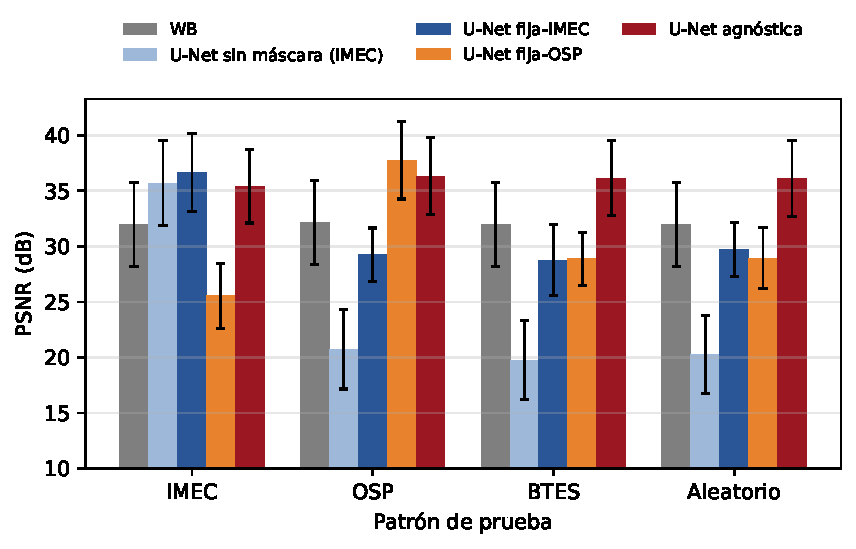
\includegraphics[width=\linewidth]{psnr_bars.pdf}
\caption{PSNR medio en las 8 escenas de prueba para cada método y patrón de
prueba (barras de error: desviación estándar entre escenas). Las redes
específicas solo funcionan bien en el patrón con que se entrenaron; la red
agnóstica (rojo oscuro) funciona bien en los cuatro.}
\label{fig:bars}
\end{figure}

\begin{table}[t]
\centering
\caption{Pruebas de hipótesis (PSNR, dB). H1: caída desde el patrón propio
de la red hasta la media de los tres patrones no vistos. H2 y H3:
diferencias pareadas por escena, como media e intervalo de confianza de
95\%. ``Escenas'': en H2, número de escenas (de 8) con brecha menor que
2\,dB / menor que 1\,dB; en H3, número de escenas en que la red agnóstica es
mejor.}
\label{tab:hyp}
\footnotesize
\setlength{\tabcolsep}{4pt}
\begin{tabular}{|l|l|c|c|}
\hline
Otra red & MSFA de prueba & Media [IC 95\%] & Escenas \\
\hline
\multicolumn{4}{|l|}{\textbf{H1}: patrón propio $-$ patrones no vistos} \\
\hline
Fija-IMEC          & 3 no vistos & 7.38  & -- \\
Fija-OSP           & 3 no vistos & 9.94  & -- \\
Sin máscara (IMEC) & 3 no vistos & 15.45 & -- \\
\hline
\multicolumn{4}{|l|}{\textbf{H2}: específica $-$ agnóstica, en el patrón de la específica} \\
\hline
Fija-IMEC & IMEC & 1.21 [0.66, 1.75] & 8 / 2 \\
Fija-OSP  & OSP  & 1.40 [0.88, 1.93] & 5 / 3 \\
\hline
\multicolumn{4}{|l|}{\textbf{H3}: agnóstica $-$ otro método, en patrones no vistos} \\
\hline
Fija-IMEC & OSP       & 7.08 [5.39, 8.77]  & 8 \\
Fija-IMEC & BTES      & 7.37 [5.54, 9.20]  & 8 \\
Fija-IMEC & Aleatorio & 6.33 [4.86, 7.80]  & 8 \\
Fija-OSP  & IMEC      & 9.89 [6.79, 12.98] & 8 \\
Fija-OSP  & BTES      & 7.25 [5.36, 9.13]  & 8 \\
Fija-OSP  & Aleatorio & 7.12 [5.27, 8.97]  & 8 \\
WB        & IMEC      & 3.44 [1.71, 5.16]  & 7 \\
WB        & OSP       & 4.20 [2.22, 6.18]  & 8 \\
WB        & BTES      & 4.16 [2.29, 6.03]  & 8 \\
WB        & Aleatorio & 4.08 [2.20, 5.95]  & 8 \\
\hline
\end{tabular}
\end{table}

\subsection{H1: las redes específicas fallan en patrones no vistos}

H1 se cumple. La red fija-IMEC alcanza 36.64\,dB en IMEC, pero solo 28.77 a
29.74\,dB en los otros patrones, una caída media de 7.38\,dB. La fija-OSP
cae 9.94\,dB, de 37.73 a 25.55--28.95\,dB. La red convencional sin máscara
cae 15.45\,dB, hasta cerca de 20\,dB. Las tres terminan bajo WB, que no
aprende nada, por 2.2 a 12.2\,dB. El error espectral crece aún más: el SAM
pasa de cerca de $4^\circ$ a $13$--$14^\circ$ en las redes fijas y a
$26$--$35^\circ$ en la red sin máscara, y con esos valores los espectros
reconstruidos sirven de poco. Que falle la red convencional era esperable,
porque no tiene acceso al patrón y en un MSFA nuevo asigna cada medición a
la banda equivocada. Las redes fijas son el caso más interesante, porque
reciben la máscara y aun así fallan. Una red que siempre ve el mismo patrón
puede ignorar la máscara y memorizar el patrón, de modo que la máscara solo
ayuda si los patrones de entrenamiento varían.

\subsection{H2: brecha en el patrón propio de las redes específicas}

En su propio patrón, cada red específica es mejor que la agnóstica. La
brecha es de 1.21\,dB en IMEC (36.64 frente a 35.43\,dB) y de 1.40\,dB en
OSP (37.73 frente a 36.33\,dB). Ambos intervalos de 95\%, [0.66, 1.75] y
[0.88, 1.93], quedan bajo 2\,dB, así que H2 se cumple con el umbral de
2\,dB de nuestro plan de proyecto. Con el umbral de 1\,dB de la propuesta
escrita no se cumple, ya que la mayor parte de ambos intervalos está sobre
1\,dB. Por escena, la brecha es menor que 2\,dB en las 8 escenas en IMEC y
en 5 de 8 en OSP, y menor que 1\,dB en solo 2 y 3 escenas. En una escena de
IMEC la red agnóstica supera a la específica, por 0.19\,dB. La brecha en
SSIM también es pequeña (0.964 frente a 0.967 y 0.970 frente a 0.975). La
brecha espectral es algo mayor: el SAM sube de $4.18^\circ$ a $4.94^\circ$
en IMEC y de $4.14^\circ$ a $4.69^\circ$ en OSP.

También comparamos la red agnóstica con la red convencional sin máscara, que
es lo que normalmente se entrenaría para una cámara IMEC. En IMEC ambas son
casi iguales (35.43 frente a 35.70\,dB). La diferencia media de 0.27\,dB
cambia de signo entre escenas, de $-2.85$ a $+1.53$\,dB. En IMEC, entonces,
la red agnóstica rinde igual que la convencional, y además funciona en los
otros patrones.

\subsection{H3: generalización a patrones no vistos}

H3 se cumple en todos los casos. En los patrones que las redes específicas
no vieron, la red agnóstica es mejor por 6.33 a 9.89\,dB en promedio, y gana
en las 8 escenas de cada una de las seis comparaciones. También mejora a WB
por 3.44 a 4.20\,dB en promedio, en 31 de los 32 pares escena--patrón. La
excepción es \textit{stuffed toys} en IMEC (35.22 frente a 35.37\,dB), una
escena suave en la que WB ya es fuerte. La calidad de la red agnóstica casi
no cambia entre patrones (35.43 a 36.33\,dB). Igual que las redes
específicas, y como en~\cite{diaz2023}, rinde mejor con OSP que con IMEC, lo
que concuerda con el muestreo espacio-espectral más uniforme de OSP. La
fija-OSP en OSP también supera a la fija-IMEC en IMEC (37.73 frente a
36.64\,dB).

\subsection{Validación entre conjuntos de datos: entrenamiento con ARAD-1K}
\label{sec:cross}

\begin{table}[t]
\centering
\caption{Protocolo entre conjuntos de datos: entrenamiento con ARAD-1K y
prueba en las 32 escenas de CAVE (PSNR medio en dB). Subrayado: patrón de
entrenamiento propio. Negrita: mejor valor por columna.}
\label{tab:arad}
\footnotesize
\setlength{\tabcolsep}{3.5pt}
\begin{tabular}{|l|c|c|c|c|}
\hline
Método & IMEC & OSP & BTES & Aleatorio \\
\hline
WB (sin aprendizaje)      & 33.56 & 33.75 & 33.55 & 33.55 \\
U-Net sin máscara (IMEC)  & \seen{33.86} & 23.56 & 22.33 & 22.82 \\
U-Net fija-IMEC           & \seen{\textbf{36.30}} & 30.84 & 31.02 & 31.26 \\
U-Net fija-OSP            & 29.63 & \seen{\textbf{36.48}} & 30.77 & 30.76 \\
U-Net agnóstica (nuestra) & 34.97 & 35.47 & \textbf{35.29} & \textbf{35.31} \\
\hline
\end{tabular}
\end{table}

La partición de CAVE tiene solo 8 escenas de prueba, y las escenas de
entrenamiento y de prueba vienen del mismo conjunto de datos. Para comprobar
que los resultados no dependen de esto, reentrenamos las cuatro redes con
ARAD-1K, con la misma configuración, y las probamos en las 32 escenas de
CAVE (Tabla~\ref{tab:arad}). Las tres hipótesis se vuelven a cumplir. En
H1, la fija-IMEC, la fija-OSP y la red sin máscara pierden 5.26, 6.09 y
10.96\,dB en patrones no vistos y quedan bajo WB. En H2, la brecha con la
red específica es de 1.33\,dB en IMEC (IC 95\% [1.16, 1.50]) y de 1.01\,dB
en OSP ([0.75, 1.27]). Es menor que 2\,dB en 31 de 32 escenas en ambos
patrones y menor que 1\,dB en 7 y 14 escenas, así que, como antes, H2 se
cumple con 2\,dB pero no con 1\,dB. En H3, la red agnóstica supera a las
específicas en patrones no vistos por 4.05 a 5.34\,dB, en las 32 escenas de
las seis comparaciones, y a WB por 1.41 a 1.76\,dB (intervalos desde [0.37,
2.44] hasta [0.69, 2.84]). Esta vez también supera a la red sin máscara en
IMEC, por 1.10\,dB ([0.66, 1.55], 25 de 32 escenas).

La ventaja sobre WB es menor que en la partición de CAVE. En seis escenas
(\textit{cd}, \textit{clay}, \textit{superballs}, \textit{pompoms},
\textit{balloons} y \textit{stuffed toys}) la red agnóstica queda bajo WB en
los cuatro patrones, hasta por 7.2\,dB. Su SAM medio, y el de las redes
específicas en su propio patrón (11.2 a $13.4^\circ$), es cerca del doble
que el de WB ($5.5^\circ$). El problema no es exclusivo de la red agnóstica.
En esas mismas seis escenas las redes específicas también quedan bajo WB en
su propio patrón, y en las 8 escenas de prueba de la partición de CAVE las
redes entrenadas con ARAD-1K pierden entre 2.5 y 4.0\,dB respecto de las
mismas redes entrenadas con CAVE, mientras que WB no cambia. Por eso
atribuimos la pérdida al cambio de conjunto de datos. Los fondos negros de
CAVE no son la causa, ya que la mayor parte del error adicional está en
píxeles claros. Una diferencia que sí encontramos es la suavidad espectral:
normalizados por su media, los espectros de CAVE cambian entre bandas
vecinas cerca del doble que los de ARAD-1K (diferencia absoluta media de
0.195 frente a 0.100). Probablemente las redes aprenden de ARAD-1K un modelo
espectral demasiado suave para CAVE. Todas las redes comparten los mismos
datos de entrenamiento, así que la comparación entre ellas, y con ella
H1--H3, sigue siendo válida.

\subsection{Precisión por banda y fidelidad espectral}

\begin{figure*}[t]
\centering
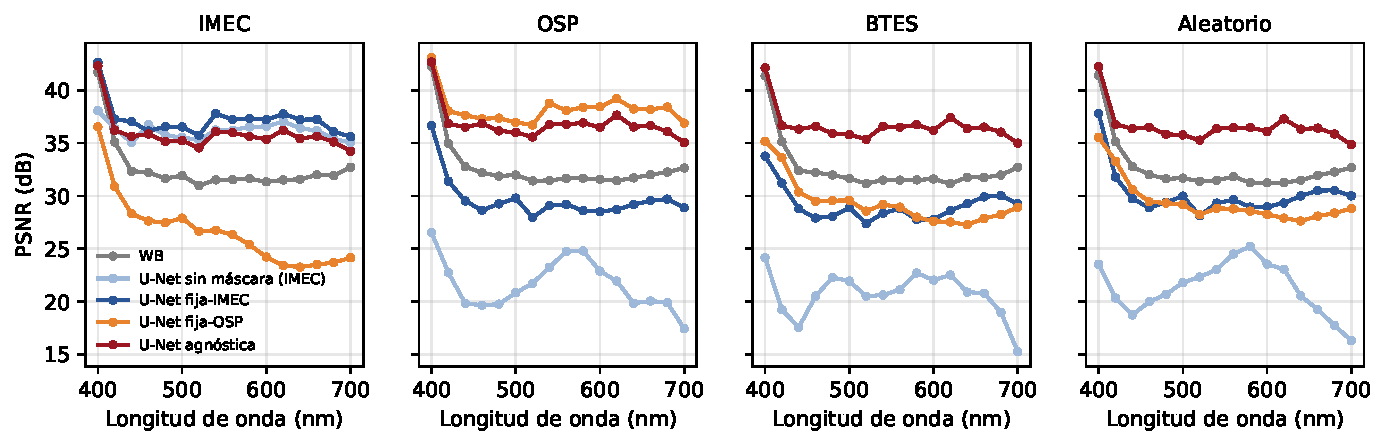
\includegraphics[width=\linewidth]{psnr_per_band.pdf}
\caption{PSNR de cada banda, promediado en las 8 escenas de prueba, para
cada patrón de prueba. La red agnóstica (rojo oscuro) da una curva plana de
35 a 37\,dB en todos los patrones. Las redes específicas solo superan a WB
en su propio patrón.}
\label{fig:bands}
\end{figure*}

La Fig.~\ref{fig:bands} muestra el PSNR por banda. Todos los métodos
alcanzan su mayor PSNR en 400\,nm, una banda oscura en CAVE con errores
absolutos pequeños. En las demás bandas, la red agnóstica se mantiene entre
35 y 37\,dB en todos los patrones, 3 a 5\,dB sobre WB. Cada red específica
es la mejor, o casi, en todas las bandas de su propio patrón, y queda bajo
WB en todas las bandas de los otros patrones. La degradación no es uniforme:
la fija-OSP en IMEC pierde precisión de manera sostenida con la longitud de
onda, de 36.5\,dB en 400\,nm a cerca de 23\,dB en 640\,nm, lo que es
coherente con bandas que se confunden entre sí. La Fig.~\ref{fig:spectra}
muestra los espectros reconstruidos de dos píxeles con OSP. WB oscila en
torno al espectro real porque las bandas vecinas se interpolan a partir de
muestras en posiciones distintas, que es la versión espectral del artefacto
zipper. La red sin máscara pierde la forma del espectro, y las redes con
máscara siguen a la referencia.

\begin{figure}[t]
\centering
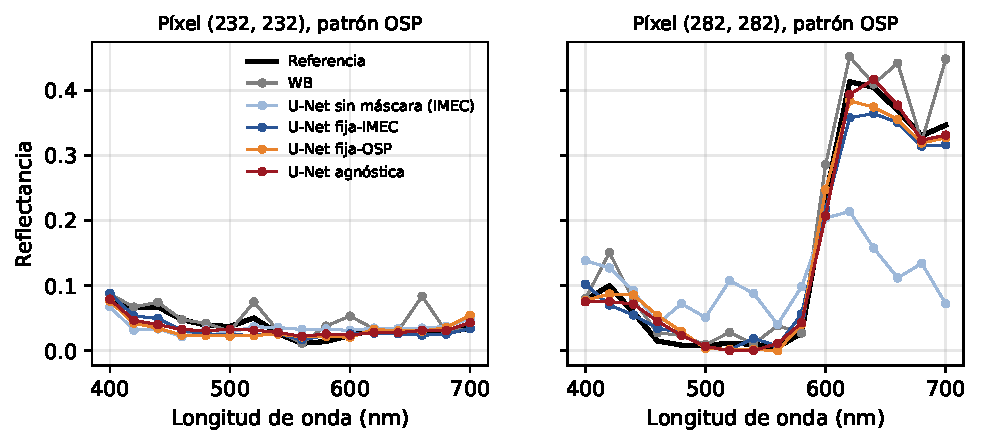
\includegraphics[width=\linewidth]{spectra.pdf}
\caption{Espectros reconstruidos de dos píxeles de la escena \textit{beads}
con el patrón OSP. WB oscila en torno a la referencia y la red sin máscara
(entrenada con IMEC) pierde la forma espectral; la red agnóstica sigue a la
referencia.}
\label{fig:spectra}
\end{figure}

\subsection{Inspección visual}

\begin{figure*}[t]
\centering
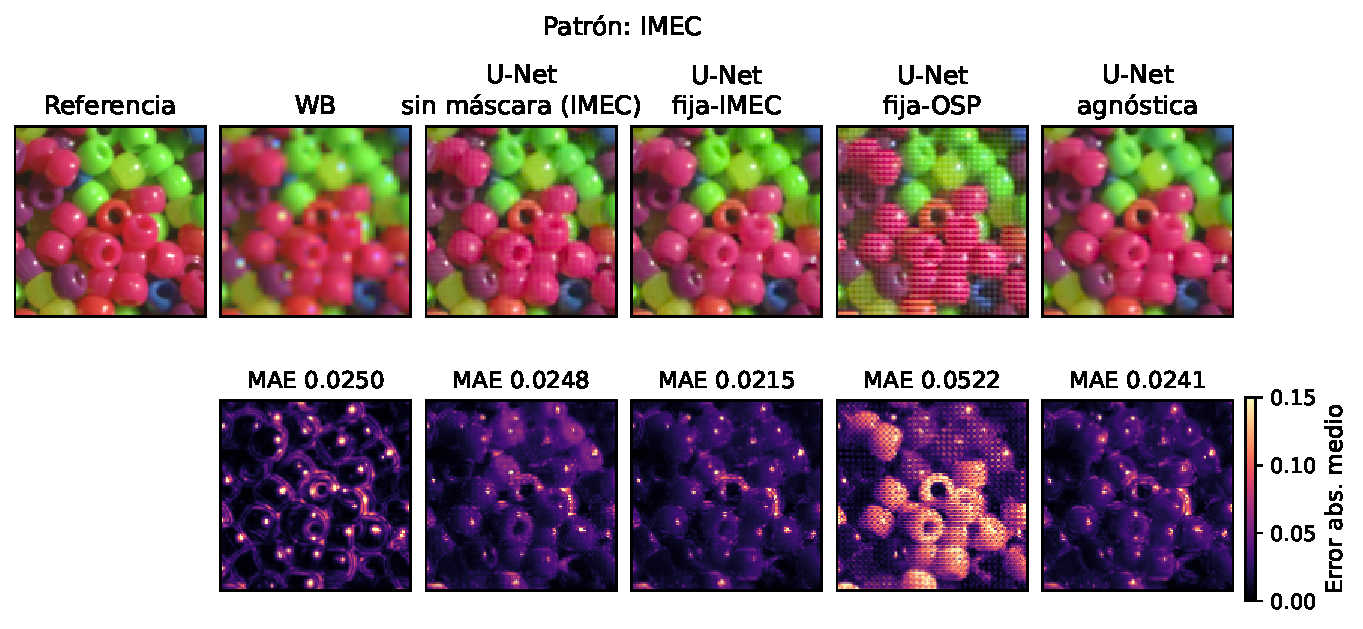
\includegraphics[width=0.49\linewidth]{visual_imec.pdf}\hfill
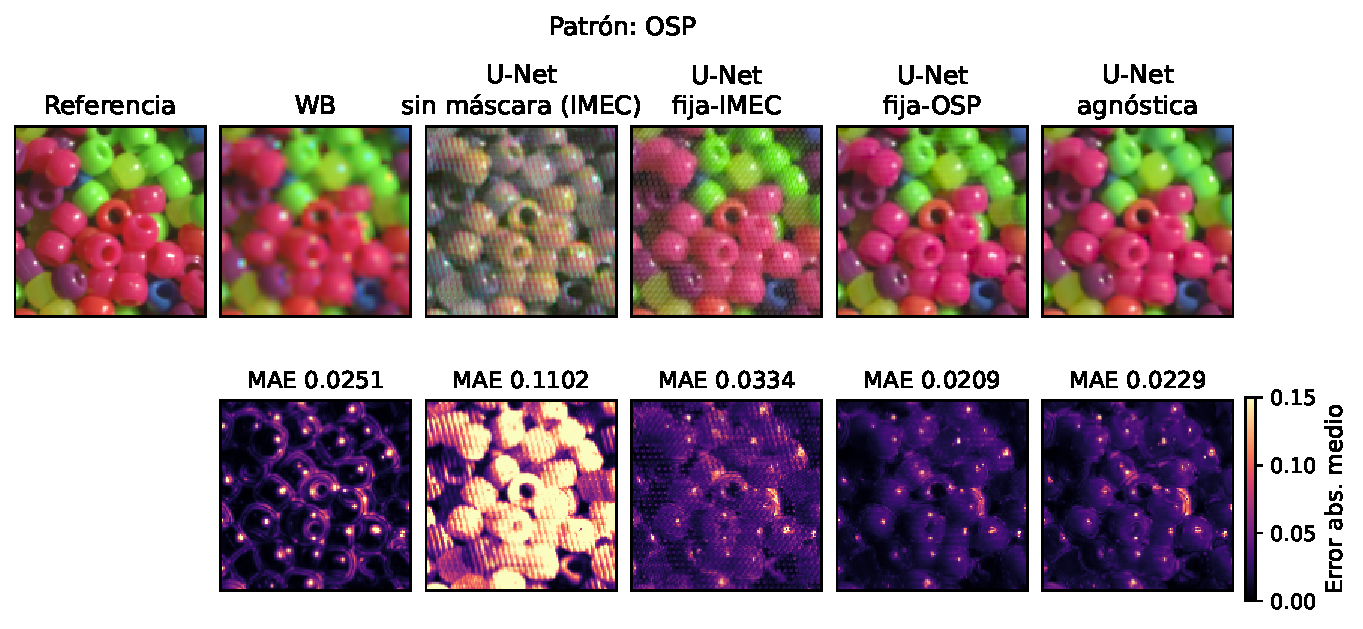
\includegraphics[width=0.49\linewidth]{visual_osp.pdf}
\caption{Recorte central de $128\times128$ de la escena de prueba
\textit{beads} con los patrones IMEC (izquierda) y OSP (derecha), en falso
color (bandas de 660, 540 y 460\,nm). Arriba: reconstrucciones. Abajo: error
absoluto medio entre bandas (MAE del recorte sobre cada mapa). En un patrón
no visto, las redes producen artefactos periódicos (fija-OSP en IMEC,
fija-IMEC en OSP) y colores falsos (sin máscara en OSP); la red agnóstica
no.}
\label{fig:visual}
\end{figure*}

La Fig.~\ref{fig:visual} muestra un recorte de \textit{beads}, la escena de
prueba más difícil (todos los métodos quedan bajo 32\,dB en ella). WB
desenfoca los bordes, y la mayor parte de su error está en los contornos y
en los brillos especulares. En un patrón no visto, las redes específicas
producen artefactos estructurados. La fija-OSP en IMEC cubre la imagen con
una grilla que tiene el período del kernel de filtros (zipper), y el error
de su recorte es el doble que el de WB (0.052 frente a 0.025). La fija-IMEC
en OSP muestra una textura periódica más débil. La red sin máscara en OSP da
colores falsos intensos, las cuentas se vuelven grisáceas y su error es más
de cuatro veces el de WB (0.110). Con la red agnóstica no vemos ni zipper ni
colores falsos, y su error (0.024 en IMEC, 0.023 en OSP) es cercano al de la
red específica en su propio patrón (0.022 y 0.021).

\subsection{Ablación de la entrada de la red}
\label{sec:ablation}

Nuestra primera red agnóstica recibía $[\Y,\M]$, como proponía el plan de
proyecto. En entrenamientos cortos aprendía mucho más lento que las redes
específicas, así que antes del entrenamiento final comparamos varias
entradas (Tabla~\ref{tab:ablation}). Estas pruebas usaron 2\,000
iteraciones y las 3 escenas de validación (nunca las de prueba), así que las
cifras son solo indicativas. Con $[\Y,\M]$, la red agnóstica queda entre 3.3
y 4.4\,dB bajo WB, y el cubo disperso, $[\Y\odot\M,\M]$, gana solo cerca de
1\,dB. También probamos dejar WB como base fija y que la red aprendiera una
corrección residual. Esa red colapsó exactamente a WB. En unas 20
iteraciones murieron todas las unidades ReLU de la última capa oculta y los
gradientes se anularon, porque el residuo objetivo es diminuto (mediana
$0.0016$) comparado con el paso de Adam; esto ocurrió incluso al inicializar
la última capa en cero. Entregar la estimación WB como \emph{entrada}
(Ec.~\eqref{eq:input}) resolvió el problema: la red agnóstica pasó de 28.3 a
34.6\,dB en IMEC, ya 2\,dB sobre WB. Nuestra interpretación es que WB hace
la parte del trabajo que depende del patrón (qué muestra pertenece a qué
banda y cómo repartirla), y la red solo tiene que aprender un refinamiento
que no depende del patrón. Esta entrada también fue mejor para las redes
específicas (fija-IMEC 36.12\,dB con 2\,000 iteraciones), así que la usamos
en todas las redes, que entonces se diferencian solo en sus patrones de
entrenamiento.

\begin{table}[t]
\centering
\caption{Ablación de la entrada de la red agnóstica (pruebas cortas:
2\,000 iteraciones, 3 escenas de validación, PSNR en dB). Solo indicativa;
las redes finales se entrenaron 10 veces más.}
\label{tab:ablation}
\footnotesize
\setlength{\tabcolsep}{3.5pt}
\begin{tabular}{|l|c|c|c|c|}
\hline
Entrada / método & IMEC & OSP & BTES & Aleatorio \\
\hline
WB (sin aprendizaje)          & 32.60 & 32.66 & 32.60 & 32.60 \\
\hline
$[\Y,\M]$ (propuesta)          & 28.26 & 28.45 & 29.11 & 29.34 \\
$[\Y\odot\M,\M]$              & 29.89 & 29.80 & 29.75 & 29.86 \\
WB + residuo aprendido        & 32.60 & 32.66 & 32.60 & 32.60 \\
$[\wb,\Y\odot\M,\M]$ (nuestra) & \textbf{34.61} & \textbf{35.07} & \textbf{35.02} & \textbf{34.89} \\
\hline
\end{tabular}
\end{table}

Las pruebas cortas también explican por qué las redes específicas reciben la
máscara. Una U-Net con dos submuestreos es equivariante a desplazamientos de
4 píxeles, pero OSP se repite cada 16 filas, así que sin la máscara la red no
puede saber en qué fase de filas del patrón se encuentra. Una red fija-OSP
sin máscara rindió igual con el patrón desplazado 4 filas (33.40 frente a
33.42\,dB), y la máscara la mejoró en 1.45\,dB. Sin la máscara, la red
específica de OSP sería más débil de lo que debería y parte de la brecha de
H2 quedaría oculta.

\subsection{Comportamiento del entrenamiento}

En la partición de CAVE, el PSNR de validación (las curvas están en el
repositorio) deja de mejorar en cerca de 35.5\,dB después de 8\,000
iteraciones para la fija-IMEC, en 34.8\,dB después de 13\,000 para la red
agnóstica y en 37.3\,dB después de 15\,000 para la fija-OSP, mientras la
pérdida de entrenamiento sigue bajando. Con 10 veces más iteraciones que en
las pruebas cortas, la brecha de H2 en IMEC solo pasó de cerca de 1.5 a
1.21\,dB, y con diez veces más escenas de entrenamiento (ARAD-1K) las
brechas son parecidas (1.33 y 1.01\,dB). No esperamos que más iteraciones o
más datos por sí solos cierren la brecha; el límite podría ser la capacidad
de la red.

% ==========================================================================
\section{Discusión}
\label{sec:discussion}
% ==========================================================================

\textbf{Implicancias.} En un MSFA nuevo, una red entrenada para un patrón es
peor que la interpolación bilineal y produce artefactos zipper y colores
falsos. Una sola red que recibe la máscara y se entrena con patrones
aleatorios balanceados evita esto en cuatro MSFA bastante distintos,
incluida una retícula no periódica (OSP), y pierde entre 1.0 y 1.4\,dB
frente a una red específica en el patrón de esa red. Vemos tres usos para
una red así. Permite comparar MSFA candidatos sin entrenar una red por
patrón, lo que responde a la limitación señalada en~\cite{diaz2023}. Puede
servir a sensores con distintas disposiciones de filtros, o a un sensor cuya
disposición difiere un poco de su diseño nominal. Y cuando la cámara es
fija, es un punto de partida razonable para ajustarla a ese patrón, aunque
no lo probamos.

\textbf{Por qué funciona.} Nuestros resultados sugieren que hacen falta dos
condiciones. La red tiene que conocer el patrón, por medio de la máscara o
de una interpolación que dependa del patrón; si no, no puede distinguir las
bandas en un MSFA nuevo. Además, los patrones de entrenamiento tienen que
variar; si no, la red aprende a ignorar la máscara, como muestran nuestras
redes fijas. Con patrones variados pero con la entrada $[\Y,\M]$, la red
agnóstica aprende lento. Entregar WB como entrada es una forma simple de
cumplir ambas condiciones: la convolución normalizada, un operador clásico
que sirve para cualquier patrón, se encarga de la geometría del patrón, y la
red aprende el modelo de las imágenes.

\textbf{Originalidad.} El entrenamiento con patrones aleatorios ya se mostró
para CFA RGB~\cite{bourrier2022}, condicionar con máscaras aleatorias es
habitual en \emph{inpainting}~\cite{liu2018} y la convolución
normalizada~\cite{knutsson1993} es anterior al aprendizaje profundo. Lo que
aportamos es el uso de estas ideas en demosaicking MSFA de 16 bandas, donde
las redes todavía se entrenan por patrón~\cite{feng2021,diaz2023}, y un
análisis de lo que necesitan en este caso más difícil. En nuestra ablación,
una entrada de cubo disperso como la que se usa en RGB
en~\cite{bourrier2022} aprende demasiado lento con 16 bandas, y entregar como
entrada una interpolación que depende del patrón lo soluciona. Además
medimos de forma controlada el costo de depender del patrón, con redes
específicas y una red agnóstica que solo se diferencian en sus patrones de
entrenamiento.

\textbf{Limitaciones.} (1) \emph{Datos}: el protocolo principal prueba en
solo 8 escenas de CAVE. El protocolo entre conjuntos de datos confirma H1--H3
en 32 escenas, pero muestra que todos los métodos aprendidos pierden
precisión, sobre todo espectral, cuando los datos de prueba difieren de los
de entrenamiento; con entrenamiento en ARAD-1K, la ventaja sobre WB baja a
1.4--1.8\,dB y desaparece en 6 de 32 escenas. (2) \emph{Simulación}:
suponemos filtros ideales de banda angosta y ausencia de ruido. Los filtros
IMEC reales se traslapan espectralmente y los sensores reales agregan ruido,
lo que haría el problema más difícil para todos los métodos.
(3) \emph{Patrones}: todos los patrones de prueba y de entrenamiento tienen
16 bandas y una banda por bloque de $4\times4$. No probamos patrones con
bandas repetidas ni otros tamaños de kernel, que la red agnóstica podría no
manejar. (4) \emph{Líneas base}: comparamos redes con la misma
arquitectura, lo que aísla el efecto de los patrones de entrenamiento, pero
no nos comparamos con redes de demosaicking del estado del arte como TRevSCI
o MCAN, ni con métodos clásicos más fuertes como PPID. Como referencia,
TRevSCI reporta 35.8, 37.6 y 38.8\,dB en IMEC, BTES y OSP~\cite{diaz2023},
pero con otro protocolo, así que esas cifras no son directamente comparables
con las nuestras. (5) \emph{Estadística}: cada red se entrenó una sola vez,
con una semilla, así que no medimos la variación entre entrenamientos.

\textbf{Trabajo futuro.} Nos gustaría entrenar con varios conjuntos de datos
para reducir la brecha entre ellos, agregar ruido y respuestas reales de los
filtros, probar patrones de otros tamaños y con bandas repetidas, ajustar la
red agnóstica a un patrón fijo, probar una red más grande para reducir la
brecha de H2 y usar la red agnóstica como evaluador rápido dentro de un
ciclo de diseño de MSFA.

% ==========================================================================
\section{Conclusión}
\label{sec:conclusion}
% ==========================================================================

Estudiamos si una sola red de demosaicking aprendida puede servir para
cualquier arreglo de filtros multiespectral. Las redes entrenadas para un
solo patrón, con o sin la máscara como entrada, pierden entre 7.4 y
15.5\,dB en patrones no vistos y quedan bajo la interpolación bilineal (H1).
Una U-Net que recibe una estimación bilineal, las mediciones dispersas y la
máscara, y que se entrena con patrones aleatorios balanceados, queda a 1.2
o 1.4\,dB de una red específica en el patrón de esa red (H2 con umbral de
2\,dB, aunque no con 1\,dB) y supera a las redes específicas por 6.3 a
9.9\,dB y a la interpolación bilineal por 3.4 a 4.2\,dB en patrones no
vistos (H3). Entrenar con ARAD-1K y probar en las 32 escenas de CAVE
confirma las tres hipótesis, aunque el cambio de conjunto de datos perjudica
a todos los métodos aprendidos y reduce la ventaja sobre la interpolación
bilineal a 1.4--1.8\,dB. La decisión de diseño que hizo esto posible fue
entregar a la red una interpolación que depende del patrón. Así, una sola
red puede reemplazar a una red por patrón con un costo moderado en
precisión, lo que facilitaría usar demosaicking aprendido en el diseño de
MSFA y en cámaras con distintas disposiciones de filtros.

% ==========================================================================
\section{Datos, código y agradecimientos}
\label{sec:ack}
% ==========================================================================

Todo el código (simulador, líneas base, redes, entrenamiento, evaluación y
figuras) y todos los resultados de este informe están en el repositorio
{\small\url{https://github.com/GonzaMichea/Multiespectral-Demosaicking}}.
Las tablas y figuras se generan a partir de los archivos de
\texttt{results/} y \texttt{results\_arad/}, y ambos protocolos se pueden
reproducir con \texttt{scripts/run\_all.sh}. Agradecemos a los autores de
los conjuntos de datos CAVE~\cite{yasuma2010} y ARAD-1K~\cite{arad2022}, y a
Diaz et al.~\cite{diaz2023} por su código MATLAB público, que usamos para
verificar nuestros patrones y nuestra línea base WB. El software se basa en
PyTorch~\cite{paszke2019}, NumPy~\cite{harris2020},
SciPy~\cite{virtanen2020}, scikit-image~\cite{vanderwalt2014} y
Matplotlib~\cite{hunter2007}.

% Referencias.
% ------------
% Letra más chica en las referencias, como en las revistas IEEE.
\begingroup
\small
\bibliographystyle{IEEEbib}
\bibliography{strings,refs}
\endgroup

\end{document}
